\chapter{Railway Network Analyzer (RNA)}
    \label{sec:RNA}

    El sistema ferroviario consta de diversos elementos que incluyen la infraestructura, sensores, actuadores  e interfaces visuales con los conductores. Todos estos elementos se interrelacionan y funcionan en conjunto dentro del sistema de señalamiento y el sistema de enclavamiento. Cada uno de estos elementos y como se relacionan se encuentran definido en el formato railML. 

    El RNA deberá procesar cualquier archivo compatible con railML, detectar cada elemento junto a sus propiedades y como están conectados dentro de la red ferroviaria. En base a esta información, que define la infraestructura, es decir, las características estáticas de la red, el RNA deberá detectar los puntos críticos. Cada elemento ferroviario, según corresponda a cada elemento, será protegido por una serie de semáforos. La conjunción de todos estos semáforos probablemente dará lugar a superposiciones o contradicciones que luego serán simplificadas por el RNA antes de su resultado final.

    En base al señalamiento generado, el RNA debe detectar todas las rutas posibles y generar una nueva tabla de enclavamientos. De existir un señalamiento previo, deberá compararlos y verificar que todas las rutas originales pueden ser generadas combinando una o mas de las rutas nuevas. Adicionalmente, el RNA validará que el señalamiento cumple los principios establecidos en la Sección \ref{sec:principios} y que la sintaxis del archivo railML obtenido es correcta.    

    \section{Biblioteca RailML}
	\label{sec:Biblioteca}
	
    El primer paso en el desarrollo del RNA es contar con una biblioteca que permita generar un objeto equivalente uno a uno con el estándar railML y luego exportar esa información en un nuevo archivo railML. Como ya se mencionó en la Sección \ref{sec:railML}, el estándar railML define cinco clases de objetos principales: \textit{Common}, \textit{Infraestructure}, \textit{Interlocking}, \textit{RollingStock} y \textit{Timetable}. 

    La clase \textit{Common} contiene 109 clases, todas ellas utilizadas para definir características generales e invariantes para la red. Por ejemplo, podemos encontrar la clase \textit{Concessionaire} que define quien tiene la concesión de la red, la clase \textit{tBrakeType} que define el tipo de frenos aceptados en esa red, la clase tVoltage que define la tensión de la red o la clase \textit{PublicHolidayPeriodRule} que define el período de vacaciones de los operarios de la red, entre otros factores. Esta clase es obligatoria para todos los archivos en formato railML, por lo tanto es necesaria para el funcionamiento del RNA, aunque no se extraigan datos de la misma.

    La clase \textit{Infraestructure} incluye  231 clases, todas ellas enfocadas en definir las características estáticas de cada elemento ferroviario, como su posición, dimensiones y demás parámetros invariantes en el tiempo. Entre ellas podemos encontrar la clase \textit{Tracks} (ver Sección \ref{sec:tracks}), \textit{Borders} (ver Sección \ref{sec:bufferstop}), \textit{BufferStops} (ver Sección \ref{sec:bufferstop}), \textit{LevelCrossingsIS} (ver Sección \ref{sec:crossing}), \textit{TrackDetectionElement} (ver Sección \ref{sec:detectors}), \textit{Platforms} (ver Sección \ref{sec:platform}), \textit{SwitchesIS} (ver Sección \ref{sec:switches}) y \textit{SignalsIS} (ver Sección \ref{sec:signals}), entre otras. Adicionalmente incluye dos clases fundamentales para el análisis de redes de grafos: \textit{netElement} y \textit{netRelation}, ambas discutidas en la Sección \ref{sec:grafos}. En el caso de hacer análisis a nivel "mesoscópico" y "macroscópico" se tienen, además, las clases \textit{Line}, \textit{OperationalPoint} y \textit{Network}, no cubiertas en este trabajo, ya que la información obtenida en estos niveles es redundante con la obtenida a nivel "microscópico".
	
    La clase \textit{Interlocking} incluye 156 clases, todas ellas enfocadas en definir las características dinámicas de los elementos ferroviarios que las posean. Entre ellas podemos encontrar \textit{LevelCrossingsIL} (ver Sección \ref{sec:crossing}) y \textit{SwitchesIL} (ver Sección \ref{sec:switches}), necesarias tanto para el RNA como para el ACG. Adicionalmente, se encuentran las clases relacionadas a la tabla de enclavamientos y las rutas, como \textit{Routes}, \textit{CombinedRoutes}, \textit{ConflictingRoutes}, \textit{RoutesRelations},  y muchas otras referidas explícitamente a rutas, como \textit{SignalsIL}, donde se definen perfiles de velocidad para las señales. 
    
    La clase \textit{RollingStocks} incluye 30 clases, todas ellas enfocadas en definir las características de cualquier tipo de material rodante. Esta clase se divide en dos grandes clases: \textit{Vehicle} y \textit{Formations}. La primer clase contiene la información relacionada a vehículos unitarios tales como: vagón de carga, coche de pasajeros o una locomotora. La segunda clase combina los elementos de la clase \textit{Vehicle} para definir las formaciones en toda su extensión.
    
    La clase \textit{TimeTables} incluye 148 clases, todas ellas enfocadas a la logística ferroviaria. Entre sus clases podemos encontrar información respecto al tipo de formaciones que circulan en la red (clases \textit{CommercialTrains}, \textit{OperationalTrains}, \textit{TransportServicies} y \textit{Categories}), itinerarios (clases \textit{ItinerariesTT}, \textit{ConnectionTransferTimes}, \textit{CommercialSchedulings}, \textit{BaseItineraries} y \textit{TimetableScenarios}) y los anuncios a los usuarios (clases \textit{PassengerTextInfos} y \textit{Announcements}).   
    
    El RNA solamente necesita de las clases \textit{Common}, \textit{Infraestructure} e \textit{Interlocking} para funcionar, por lo que no fue necesario implementar las clases \textit{RollingStock} ni \textit{Timetable}. En total se han implementado 524 clases \cite{GITHUB}, considerando 28 clases nativas de RailTopoModel necesarias para que railML pueda interpretar los tipos de datos definidos. Todas las clases y clases mencionadas son opcionales en el estándar, salvo que se indique lo contrario, es decir, no son obligatorias para que el archivo railML se considere válido.

    En las siguientes secciones se detallarán las clases mas importantes implementadas, tal que se pueda comprender qué atributos son procesados para poder generar el señalamiento. Se comenzará con las clases relativas a la topología de la red, eje central del análisis del RNA y se proseguirá con las clases asociadas a elementos ferroviarios materiales. Simultáneamente, se profundizará en los conceptos mas destacados de cada elemento ferroviario correspondiente a esa clase, destacando cuál es el señalamiento asociado al mismo para protegerlo en base a los principios ferroviarios expuestos.

    % COMMON
    \subsection{Clase \textit{Metadata}}
    \label{sec:metadata}

    Aunque no es una clase de railML, la clase \textit{Metadata} es fundamental para que el archivo en formato railML sea válido. Se presenta el Código \ref{lst:metadata} para ilustrar los elementos presentes en la clase metadata.
    
    \begin{lstlisting}[language = XML, caption = Clase \textit{Metadata}, label = {lst:metadata}]
<metadata>
    <dc:title>Example_9.railml</dc:title>
    <dc:date>2023-10-04T10:51:21Z</dc:date>
    <dc:creator>Trenes_Argentinos</dc:creator>
    <dc:source>RaIL-AiD</dc:source>
    <dc:identifier>1</dc:identifier>
    <dc:subject>railML.org</dc:subject>
    <dc:format>0.9.5</dc:format>
    <dc:description>Ejemplo_real</dc:description>
    <dc:publisher>RaIL-AiD framework</dc:publisher>
</metadata>
    \end{lstlisting}

    Ninguno de estos campos es esencial para el análisis de la red ferroviaria, por lo que son copiados sin cambios al nuevo archivo generado. No obstante, la ausencia de alguno de estos campos o que el campo sea nulo provoca que tanto el RNA como cualquier herramienta compatible con railML considere al archivo como incompleto o corrupto.
    \subsection{Clase common}
    \label{sec:common}

    La clase Common define todos los parámetros que son invariantes a toda la red. Esta clase puede ser definida solo una vez o no definirse. Sus clases son:

    \begin{itemize}
        \item ElectrificationSystems: define la tensión y frecuencia de la red eléctrica.
        \item OrganizationalUnits: define quien administra la infraestructura, quien fabrica y opera el material rodante, quien es el cliente final, quien es el contratista y quien posee la concesión del servicio. 
        \item SpeedProfiles: define el perfil de aceleración, velocidades y frenado.
        \item Positioning: define los sistemas de posicionamiento geométrico, linear y referido a la pantalla del editor.
    \end{itemize}

    Cada uno de sus campos internos es único, pero también son opcionales. A modo de ejemplo se muestra el Código \ref{lst:common}, donde se ilustra como no todas las clases han sido definidas.
    
    \begin{lstlisting}[language = XML, caption = Clase Common , label = {lst:common}]
<common id="co_01">
    <organizationalUnits>
        <infrastructureManager id="im_01"/>
    </organizationalUnits>
    <positioning>
        <geometricPositioningSystems>
            <geometricPositioningSystem id="gps01">
                <isValid from="2023-07-26" to="2024-07-26"/>
                <name name="Example_9.railml" language="en"/>
            </geometricPositioningSystem>
        </geometricPositioningSystems>
        <linearPositioningSystems>
            <linearPositioningSystem linearReferencingMethod="absolute" 
            startMeasure="0" endMeasure="0" units="Km" id="loc-1">
                <isValid from="2023-07-26" to="2024-07-26"/>
                <name name="Loc-1" language="en"/>
            </linearPositioningSystem>
        </linearPositioningSystems>
    </positioning>
</common>
    \end{lstlisting}

    Solamente los clases OrganizationalUnits y Positioning fueron definidas, pero tanto el RNA como el estándar railML en el que el RNA se basa consideran válido a este fragmento de código. Los vectores son definidos en plural, como en el caso de geometricPositioningSystems cuyo primer, y único elemento en este caso, es geometricPositioningSystem con id="gps01". Es habitual ver estos vectores a lo largo de todo el archivo y será esencial poder determinar su dimensión para procesar correctamente los datos y contar la cantidad de elementos.

    
    % GRAFOS
    \subsection{Infraestructura y Redes de grafos}
    \label{sec:grafos}

    La clase Infraestructure define todos los elementos ferroviarios con características físicas, materiales y estáticas. Las subclases que contiene son:

    \begin{itemize}
        \item Topology: define la topología de la red mediante las subclases netElements y netRelationships. Incluye también la subclase Network para cumplir con el estándar de RailTopoModel.
        \item Geometry: define el sistema geométrico utilizado entre las subclases HorizontalCurve (en base al largo y el ángulo formado), GradientCurves (en base al largo y al gradiente ded la curva) y GeometryPoints (en base a una combinación de las dos subclases anteriores).
        \item FunctionalInfrastructure: define todos los elementos ferroviarios que el RNA analizará.
        \item PhysicalFacilities: actualmente el estándar lo define vacío, sin ninguna subclase interna salvo la subclase Any que puede ser utilizada como comodín.
        \item InfrastructureVisualizations: define las coordenadas y estructura del elemento ferroviario en base a sus subclases tRef (para indicar a que elemento afecta), SpotProjection (coordenada del elemento), LinearProjection (en caso de ser un elemento lineal) y AreaProjection (en caso de ser un elemento bidimensional).
        \item InfrastructureStates: define la validez de los datos referidos a cada elemento ferroviario.
    \end{itemize}

    Para realizar el análisis de la red, el RNA debe centrarse en tres de estas subclases: Topology (para conocer COMO es la red), FunctionalInfrastructure (para conocer QUE elementos tiene la red) y InfrastructureVisualizations (para conocer DONDE está cada elemento ferroviario).

    Empezando por la clase Topology, existen dos subclases esenciales para este análisis: la subclase netElements y la subclase netRelationships. Ambas son subclases vectores, constituidas por subclases mas pequeñas: netElement y netRelationship. Un ejemplo de la clase netElement se puede ver en el Código \ref{lst:netElement}.
    
    \begin{lstlisting}[language = XML, caption = Clase netElement , label = {lst:netElement}]
<netElement id="ne3">
    <associatedPositioningSystem id="ne3_aps01">
        <intrinsicCoordinate intrinsicCoord="0" id="ne3_aps01_ic01">
            <geometricCoordinate x="9384.050" y="0.000" positioningSystemRef="gps01"/>
        </intrinsicCoordinate>
        <intrinsicCoordinate intrinsicCoord="1" id="ne3_aps01_ic02">
            <geometricCoordinate x="7584.770" y="0.000" positioningSystemRef="gps01"/>
        </intrinsicCoordinate>
    </associatedPositioningSystem>
    <relation ref="nr_ne3ne46_swi77"/>
    <relation ref="nr_ne3ne53_swi77"/>
</netElement>
    \end{lstlisting}
    
    Los elementos mas importantes a destacar en el Código \ref{lst:netElement} son el id, el geometricCoordinate y el relation. De estos parametros podemos saber que el netElement es referido como "ne3", comienza en la coordenada (9384.050 ; 0.000) y termina en la coordenada (7584.770 ; 0.000). Además, ne3 se encuentra relacionado a los netElement ne46 y ne53 mediante un elemento referido como swi77, que mas adelante veremos que se trata de una máquina de cambios.

    Los netElement son los nodos de la red de grafos, pero estos no son puntuales, sino que son bidimensionales. De las coordenadas de ne3 podemos deducir que ne3 se encuentra definido de derecha a izquierda. Conocer la orientación del netElement será importante a la hora de definir la circulación, información necesaria para generar las rutas.

    La subclase netRelation son las aristas de la red de grafos que relacionan dos netElements entre si. En el Código \ref{lst:netRelation} se muestra un ejemplo de los netRelation que vinculan a los netElement ne3, ne46 y ne53.    
    
    \begin{lstlisting}[language = XML, caption = Clase netRelation , label = {lst:netRelation}]
<netRelation navigability="Both" positionOnA="1" positionOnB="1" id="nr_ne3ne46_swi77">
    <elementA ref="ne3"/>
    <elementB ref="ne46"/>
</netRelation>
<netRelation navigability="Both" positionOnA="1" positionOnB="1" id="nr_ne3ne53_swi77">
    <elementA ref="ne3"/>
    <elementB ref="ne53"/>
</netRelation>
<netRelation navigability="None" positionOnA="1" positionOnB="1" id="nr_ne46ne53_swi77">
    <elementA ref="ne46"/>
    <elementB ref="ne53"/>
</netRelation>
    \end{lstlisting}
    
    La primer netRelation es entre el netElement ne3 y el ne46, la segunda netRelation es entre el netElement ne3 y el ne53. Esto es consistente con los parámetros de relation que tenía el netElement ne3 en el Código \ref{lst:netElement}. Sin embargo, en el tercer netRelation vemos que existe una relación entre los netElement ne46 y ne53 pero, en este caso, el parámetro navigability es "None", a diferencia de los primeros dos que era "both". La navegabilidad es el parámetro que hace que una red de grafos tenga sentido como red ferroviaria: que exista una conexión no implica que sea físicamente utilizable por un tren, tal como se explico en la Sección \ref{sec:RTM}.
    
    % Explicar analisis de red de grafos


        \begin{algorithm}\captionsetup{labelfont={sc,bf}, labelsep=newline}
            \caption{Graph network analysis algorithm}
            \label{alg:graph_network}
            \begin{algorithmic}
                \STATE \{nodes\} $\gets$ get\_nodes(netElements)
                \STATE  order\_nodes(\{nodes\})
                \STATE \{netPaths\} $\gets$ get\_relations(\{nodes\},netRelations)
                \STATE \{neighbours\} $\gets$ get\_neighbours(\{netPaths\})
                \STATE \{switches\} $\gets$ get\_switches(\{nodes\},\{neighbours\})
                \STATE \{limits\} $\gets$ get\_limits(\{nodes\})
                \STATE analyze\_connectedness(\{netPaths\})
            \end{algorithmic}
        \end{algorithm}


\begin{algorithm}\captionsetup{labelfont={sc,bf}, labelsep=newline}
            \label{alg:connectedness}
            \caption{Connectivity algorithm}
            \begin{algorithmic}
                \STATE \{zones\} $\gets \{ \}$
                \STATE ADD first node in \{zones\}
                \FOR {node in \{nodes\}}
                    \FOR {zone in \{zones\}}
                        \IF {node not in zones[zone]}
                            \IF {neighbours(node) in zones[zone]}
                                \STATE zones[zone] ADD node
                            \ELSE
                                \STATE Define new\_zone
                                \STATE zones[new\_zone] ADD node
                            \ENDIF
                        \ENDIF
                    \ENDFOR
                \ENDFOR 
            \RETURN \{zones\}
            \end{algorithmic}
        \end{algorithm}

    \begin{algorithm}\captionsetup{labelfont={sc,bf}, labelsep=newline}
            \caption{Switches detector algorithm}
            \label{alg:switches}
            \begin{algorithmic}
                \STATE \{switches\} $\gets$ \{\}
                \IF {infrastructure.SwitchesIS != None} 
                    \FOR{i in infrastructure.SwitchesIS[0].SwitchIS}
                        \IF{i.Id not in switchesIS.keys()}
                            \STATE sw\_id $\gets$ i.Name[0].Name
                            \STATE j $\gets$ i.SpotLocation[0]
                            \STATE left\_id $\gets$ i.LeftBranch[0].NetRelationRef
                            \STATE right\_id $\gets$ i.RightBranch[0].NetRelationRef
                            \STATE switches[sw\_id] $\gets$ \{"Node":j.NetElementRef\}
                            \STATE switches[sw\_id] $\gets$ \{"Continue":i.ContinueCourse\}
                            \STATE switches[sw\_id] $\gets$ \{"Branch":i.BranchCourse\}
                            \STATE switches[sw\_id] $\gets$ \{"Dir":j.ApplicationDirection\}
                            \STATE switches[sw\_id] $\gets$ \{"LeftBranch":j.left\_id\}
                            \STATE switches[sw\_id] $\gets$ \{"RightBranch":j.right\_id\}
                        \ENDIF
                    \ENDFOR
                \ENDIF
                \STATE visual\_data $\gets$ visualization.Visualization
                \IF {visual\_data != None}
                    \FOR {i in  visual\_data[0].SpotElementProjection}
                        \STATE sw\_id $\gets$ i.Name[0].Name
                        \IF {"Sw" in sw\_id}
                            \STATE pos\_x $\gets$ int(i.Coordinate[0].X)
                            \STATE pos\_y $\gets$ int(i.Coordinate[0].Y)
                            \STATE switches[sw\_id] $\gets$ \{"Position":[pos\_x,-pos\_y]\}
                        \ENDIF 
                    \ENDFOR
                \ENDIF
            \RETURN switchesIS
            \end{algorithmic}
        \end{algorithm}

    %% Identificar nodos y aristas
    %% Identificar orientaciones
    %% Detectar conexidad
    %% Detectar si es una red ferroviaria o no


    \begin{algorithm}[hbt!]
        \caption{Level crossing algorithm}\label{alg:LC}
        \DontPrintSemicolon
        %\SetAlgoLined
        \SetNoFillComment
        \LinesNotNumbered 
        \For { netElement WITH LevelCrossing }
        {
            \tcc{Before reaching level crossing}
            [Signals] $\gets$ ADD circulation signal $>>>$\;
            \tcc{After leaving level crossing}
            [Signals] $\gets$ ADD circulation signal $<<<$\;
        }
        \KwResult{[Signals]} 
    \end{algorithm}



    
    
    En las siguientes subsecciones se analizaran en conjunto los elementos ferroviario descriptos en las subclases FunctionalInfrastructure y InfrastructureVisualizations.
    
     % ELEMENTOS
    \subsection{Vías}
	\label{sec:tracks}
	
    Las vías férreas son el elemento ferroviario mas esencial, son la columna vertebral de la infraestructura ferroviaria. Estas constituyen el sitio por el cual se desplazan los trenes, definiendo no solo la dirección del desplazamiento, sino también restringiendo el dominio del tren. Esto lo diferencia de otros medios de transporte como el automóvil que, aún teniendo una carretera, puede moverse por fuera de esta.

    Las vías se encuentran separadas por una distancia fija que se mide desde sus caras internas, denominada trocha (Figura \ref{fig:vias_1}). Solamente las formaciones compatibles con ese parámetro de trocha pueden circular por el tendido ferroviario. El valor de la trocha puede variar entre las denominadas trocha angosta (600 a 1372 mm, estándar imperial británico) y trocha ancha (1520 a 2140 mm, estándar ruso, indio, ibérico, irlandés). Se estableció el valor intermedio de 1435 mm como valor de trocha internacional, usado ampliamente en Europa, Norteamérica y Oceanía.

    \begin{figure}[H]
        \centering
        \includegraphics[width=1\textwidth]{Figuras/trocha.png}
        \centering\caption{Vías ferroviarias y trocha.}
        \label{fig:vias_1}
    \end{figure}
    
    Existen limitaciones logísticas y físicas por las cuales el tendido ferroviario no puede ser un continuo rígido. En primer lugar, las vías deben ser de un tamaño acotado, tal que puedan transportarse a la locación donde serán instaladas en tramos rectos o curvos. En segundo lugar, la dilatación y contracción de las vías debido a los cambios de temperatura añaden una restricción respecto a la distancia mínima que deben tener entre las mismas. De lo contrario, la dilatación del material puede provocar daños irreparables a la infraestructura y estos, a su vez, ser motivo de descarrilamientos, como ya ha ocurrido en los comienzos de la industria ferroviaria \cite{ACCIDENTE}. 
    
    Cada vía puede ser clasificada en dos grupos: vías ascendentes o vías descendentes (ver Figura \ref{fig:vias_2}). Las ascendentes son aquellas por las cuales los trenes circulan únicamente en la dirección del kilometraje en sentido creciente. Las descendentes son aquellas por las cuales los trenes circulan únicamente en la dirección del kilometraje en sentido decreciente \cite{RITO}. 

    \begin{figure}[H]
        \centering
        \includegraphics[width=1\textwidth]{Figuras/ascDesc.png}
        \centering\caption{Vías ascendentes y descendentes.}
        \label{fig:vias_2}
    \end{figure}

    El kilómetro cero es la estación principal de la línea ferroviaria, como pueden ser las terminales de Plaza Constitución (para la línea Roca), Once de septiembre (para la línea Sarmiento) y Retiro (para las líneas Mitre y San Martín).  Existen vías de maniobra que pueden ser tanto ascendentes como descendentes. Estas vinculan, mediante un cambio de vías, una sección ascendente con otra descendente, en la cual los trenes deben circular a una velocidad reducida. 

    Las vías se agrupan en secciones que, por cuestiones de seguridad y logística, se establece que solo pueden ser utilizadas por un tren a la vez. Estas secciones pueden ser de varios kilómetros en zonas rurales o unos pocos cientos de metros en zonas urbanas, donde la red necesita una mayor granularidad debido a la densidad del tráfico ferroviario en las grandes urbes.

    En railML las vías son elementos ferroviarios físicos, representados por la clase track, ilustrada en el Código \ref{lst:track}. Esta clase se encuentra definida dentro del vector de clases tracks, dentro de la clase functionalInfrastructure, dentro de la clase infrastructure.

    \begin{lstlisting}[language = XML, caption = Clase track , label = {lst:track}]
    <track type="mainTrack" infrastructureManagerRef="im_01" mainDirection="both" id="trk2">
        <trackBegin ref="bus5"/>
        <trackEnd ref="swi77"/>
        <length value="1799.28" type="physical"/>
        <designator register="_Example" entry="TRACK track2"/>
        <linearLocation applicationDirection="both" id="trk2_lloc01">
            <associatedNetElement netElementRef="ne3" keepsOrientation="true"/>
        </linearLocation>
        <name name="track2" language="en"/>
    </track>
    \end{lstlisting}
    
    Las vías en railML se definen entre dos elementos ferroviarios físicos. En este caso, la vía indicada como trk2 se encuentra definida entre el BufferStop bus5 (ver Sección \ref{sec:bufferstop}) y la máquina de cambios swi77 (ver Sección \ref{sec:switches}). Esta clase define, además, el largo de la vía y el netElement al cual están asociadas, en este caso, el netElement ne3. Es natural confundirse tracks y netElements, porque son términos casi equivalentes, pero un track representa un elemento físico y un netElement engloba de manera abstracta una porción del trazado de vías. Es decir, una vía puede dividirse en varios netElements, pero un netElement solo se asocia a una vía.
    \subsection{Fin de via}

\lipsum[1]
    \subsection{Sistemas de detección de formaciones ferroviarias}
    \label{sec:detectors}
    
    Es de vital importancia que el sistema pueda determinar la posición de un tren dentro del tendido ferroviario. De esta manera, poder habilitar la circulación en secciones donde no exista peligro de colisión con otros formaciones o, por el contrario, detener la marcha de las formaciones anteriores para evitar accidentes. Existen diversas maneras de detectar la posición de un tren, entre ellas el uso de circuitos de vía y contadores de ejes (Figura \ref{fig:deteccion_1}). 

    \begin{figure}[H]
        \centering
        \includegraphics[width=1\textwidth]{Figuras/detector}
        \centering\caption{Circuito de vía (01) y contador de ejes (AxC01).}
        \label{fig:deteccion_1}
    \end{figure}

    Los circuitos de vía (Figura \ref{fig:deteccion_2}) son dispositivos eléctricos que aplican una diferencia de potencial entre los rieles. Cuando una formación ingresa a la sección, sus ruedas metálicas cortocircuitan ambos rieles. El cortocircuito es detectado por el relé, que a su vez, reporta el estado al resto del sistema. 

    \begin{figure}[H]
        \centering
        \includegraphics[width=1\textwidth]{Figuras/circuitoVia}
        \centering\caption{Circuito de vía libre y ocupado.}
        \label{fig:deteccion_2}
    \end{figure}

    En caso de que la alimentación se interrumpa, el cableado sufra alguna falla, vandalismo, inundación, o que efectivamente una formación ocupe la sección, el circuito de vía reportará que la sección se encuentra ocupada. De esta manera, solo es posible recibir un reporte de sección desocupada cuando la sección efectivamente se encuentre desocupada. A este principio se le denomina fail-safe \cite{Paper_5,Paper_94,Paper_95,Paper_96}. Es decir, si por alguna razón algo falla, el sistema adopta la condición más restrictiva, mitigando la posibilidad de una situación peligrosa. 
    
    Existe una discontinuidad entre los rieles denominado juntura, que permite la expansión de los mismos al ser sometidos a altas temperaturas sin que los rieles se doblen y provoquen daños a la infraestructura. Los circuitos de vía, se relacionan directamente a las junturas entre las vías, modelados por la clase \textit{railJoint} en railML.  Esta discontinuidad eléctrica es lo que limita la acción del circuito de vía a la región entre dos junturas.

    En el código \ref{lst:trackCircuit} podemos ver un ejemplo de la clase \textit{tvdSection} dentro de la clase \textit{interlocking}, que incluye a la clase \textit{assetsForIL} y estos, a su vez, a la clase vector de \textit{tvdSections}. Esta clase posee un id (tvd7), la tecnología utilizada (en este caso \textit{trackCircuit}, circuito de vía) y los límites donde el circuito de vía es válido: los \textit{bufferStop} bus1 y bus2.

    \begin{lstlisting}[language = XML, caption = Clase \textit{TrackCircuit} , label = {lst:trackCircuit}]
    <tvdSection id="tvd7" partialRouteReleaseDelay="PT4S" residualRouteCancellationDelay="PT90S" technology="trackCircuit" isBerthingTrack="false">
        <designator register="Example" entry="01"/>
        <hasDemarcatingBufferstop ref="bus2"/>
        <hasDemarcatingBufferstop ref="bus1"/>
    </tvdSection>
    \end{lstlisting}

    Los sistemas contadores de ejes (Figura \ref{fig:deteccion_2}) consisten en sensores pasivos instalados en la cara interna de unos de los rieles y un sistema externo de procesamiento de datos. Estos sistemas no dependen de la aplicación de tensiones en la vía. Además, no solo permiten detectar la presencia de una formación, sino que también pueden usarse para medir la integridad de la formación, si se conoce a priori la cantidad de ejes de la misma. 

    \begin{figure}[H]
        \centering
        \includegraphics[width=1\textwidth]{Figuras/contador}
        \centering\caption{Contadores de ejes.}
        \label{fig:deteccion_2}
    \end{figure}

    Al igual que los circuitos de vía, los sistemas contadores de eje siguen el principio de fail-safe, adoptando la condición mas restrictiva en caso de falla. Ambos sistemas pueden utilizarse en simultáneo, de ser requerido. En el código \ref{lst:axleCounter} podemos ver un ejemplo de la clase \textit{trainDetectionElement}, dentro de la clase \textit{functionalInfrastructure}, dentro de la clase \textit{infrastructure}. En este ejemplo la bclase fue definida como tipo \textit{axleCounter} (contador de eje) y se le asigna el nombre AxC01 que vemos en la Figura \ref{fig:deteccion_1}, referido al \textit{netElement} ne1. También podemos ver que este contador de ejes se activa en ambos sentidos (applicationDirection = both) y su coordenada intrínseca dentro del \textit{netElement} ne1, dentro de los dos tercios de la sección.

    \begin{lstlisting}[language = XML, caption = Clase \textit{TrainDetectionElement} , label = {lst:axleCounter}]
    <trainDetectionElement id="ac6" type="axleCounter">
        <name name="AxC01" language="en"/>
        <spotLocation id="ac6_sloc01" netElementRef="ne1" applicationDirection="both" intrinsicCoord="0.6710"/>
        <designator register="Example" entry="TRAIN DETECTION ELEMENT AxC01"/>
    </trainDetectionElement>
    \end{lstlisting}
    %\subsubsection{Automatic Train Stop (ATS)}

\lipsum[1]

    \begin{figure}[!h]
        \centering
        \includegraphics[width=1\textwidth]{Figuras/ATS}
        \centering\caption{ATS.}
        \label{fig:ATS_1}
    \end{figure}

\lipsum[1]
    \subsection{Plataformas}

\lipsum[1]
    \subsection{Cruces de via}

\lipsum[1]
    \subsection{Cambios de vías}
    \label{sec:switches}
 	Un cambio de vías es un elemento ferroviario dinámico, que puede adoptar diferentes posiciones que modifican la topología de la red. Una formación por si sola no puede hacer mas que avanzar o retroceder, pero utilizando un cambio de vías es posible trazar nuevos caminos en el tendido ferroviario, modificando la posición de los cambios de vías.
 	
 	Los cambios de vías pueden ser simples, dobles o en tijeras. Las posiciones que pueden adoptar se visualizan en la Figura \ref{fig:cambios_0}. Un cambio de vías simple permite dos circulaciones posibles, una por vía principal y otra por vía secundaria. Un cambio de vías dobles permite cuatro circulaciones posibles, todas de igual prioridad. Un cambio de vías en tijeras permite dos circulaciones posibles, ambas principales.
 	
 	\begin{figure}[H]
 		\centering
 		\includegraphics[width=1\textwidth]{Figuras/circulacion.png}
 		\centering\caption{Circulaciones posibles en cambios de vías.}
 		\label{fig:cambios_0}
 	\end{figure}
 	
 	El sistema de enclavamientos modifica la posición de los cambios de vías por medio de una máquina de cambios. Una máquina de cambios (Figura \ref{fig:cambios_1}) es un mecanismo utilizado para permitir el paso de las formaciones de una vía a una ramificación del recorrido principal. Esto se realiza mediante el movimiento de la aguja del cambio (riel móvil) hacia su respectiva contraaguja (riel fijo) hasta obtener un adecuado acoplamiento que permita la circulación de la formación.

    \begin{figure}[H]
        \centering
        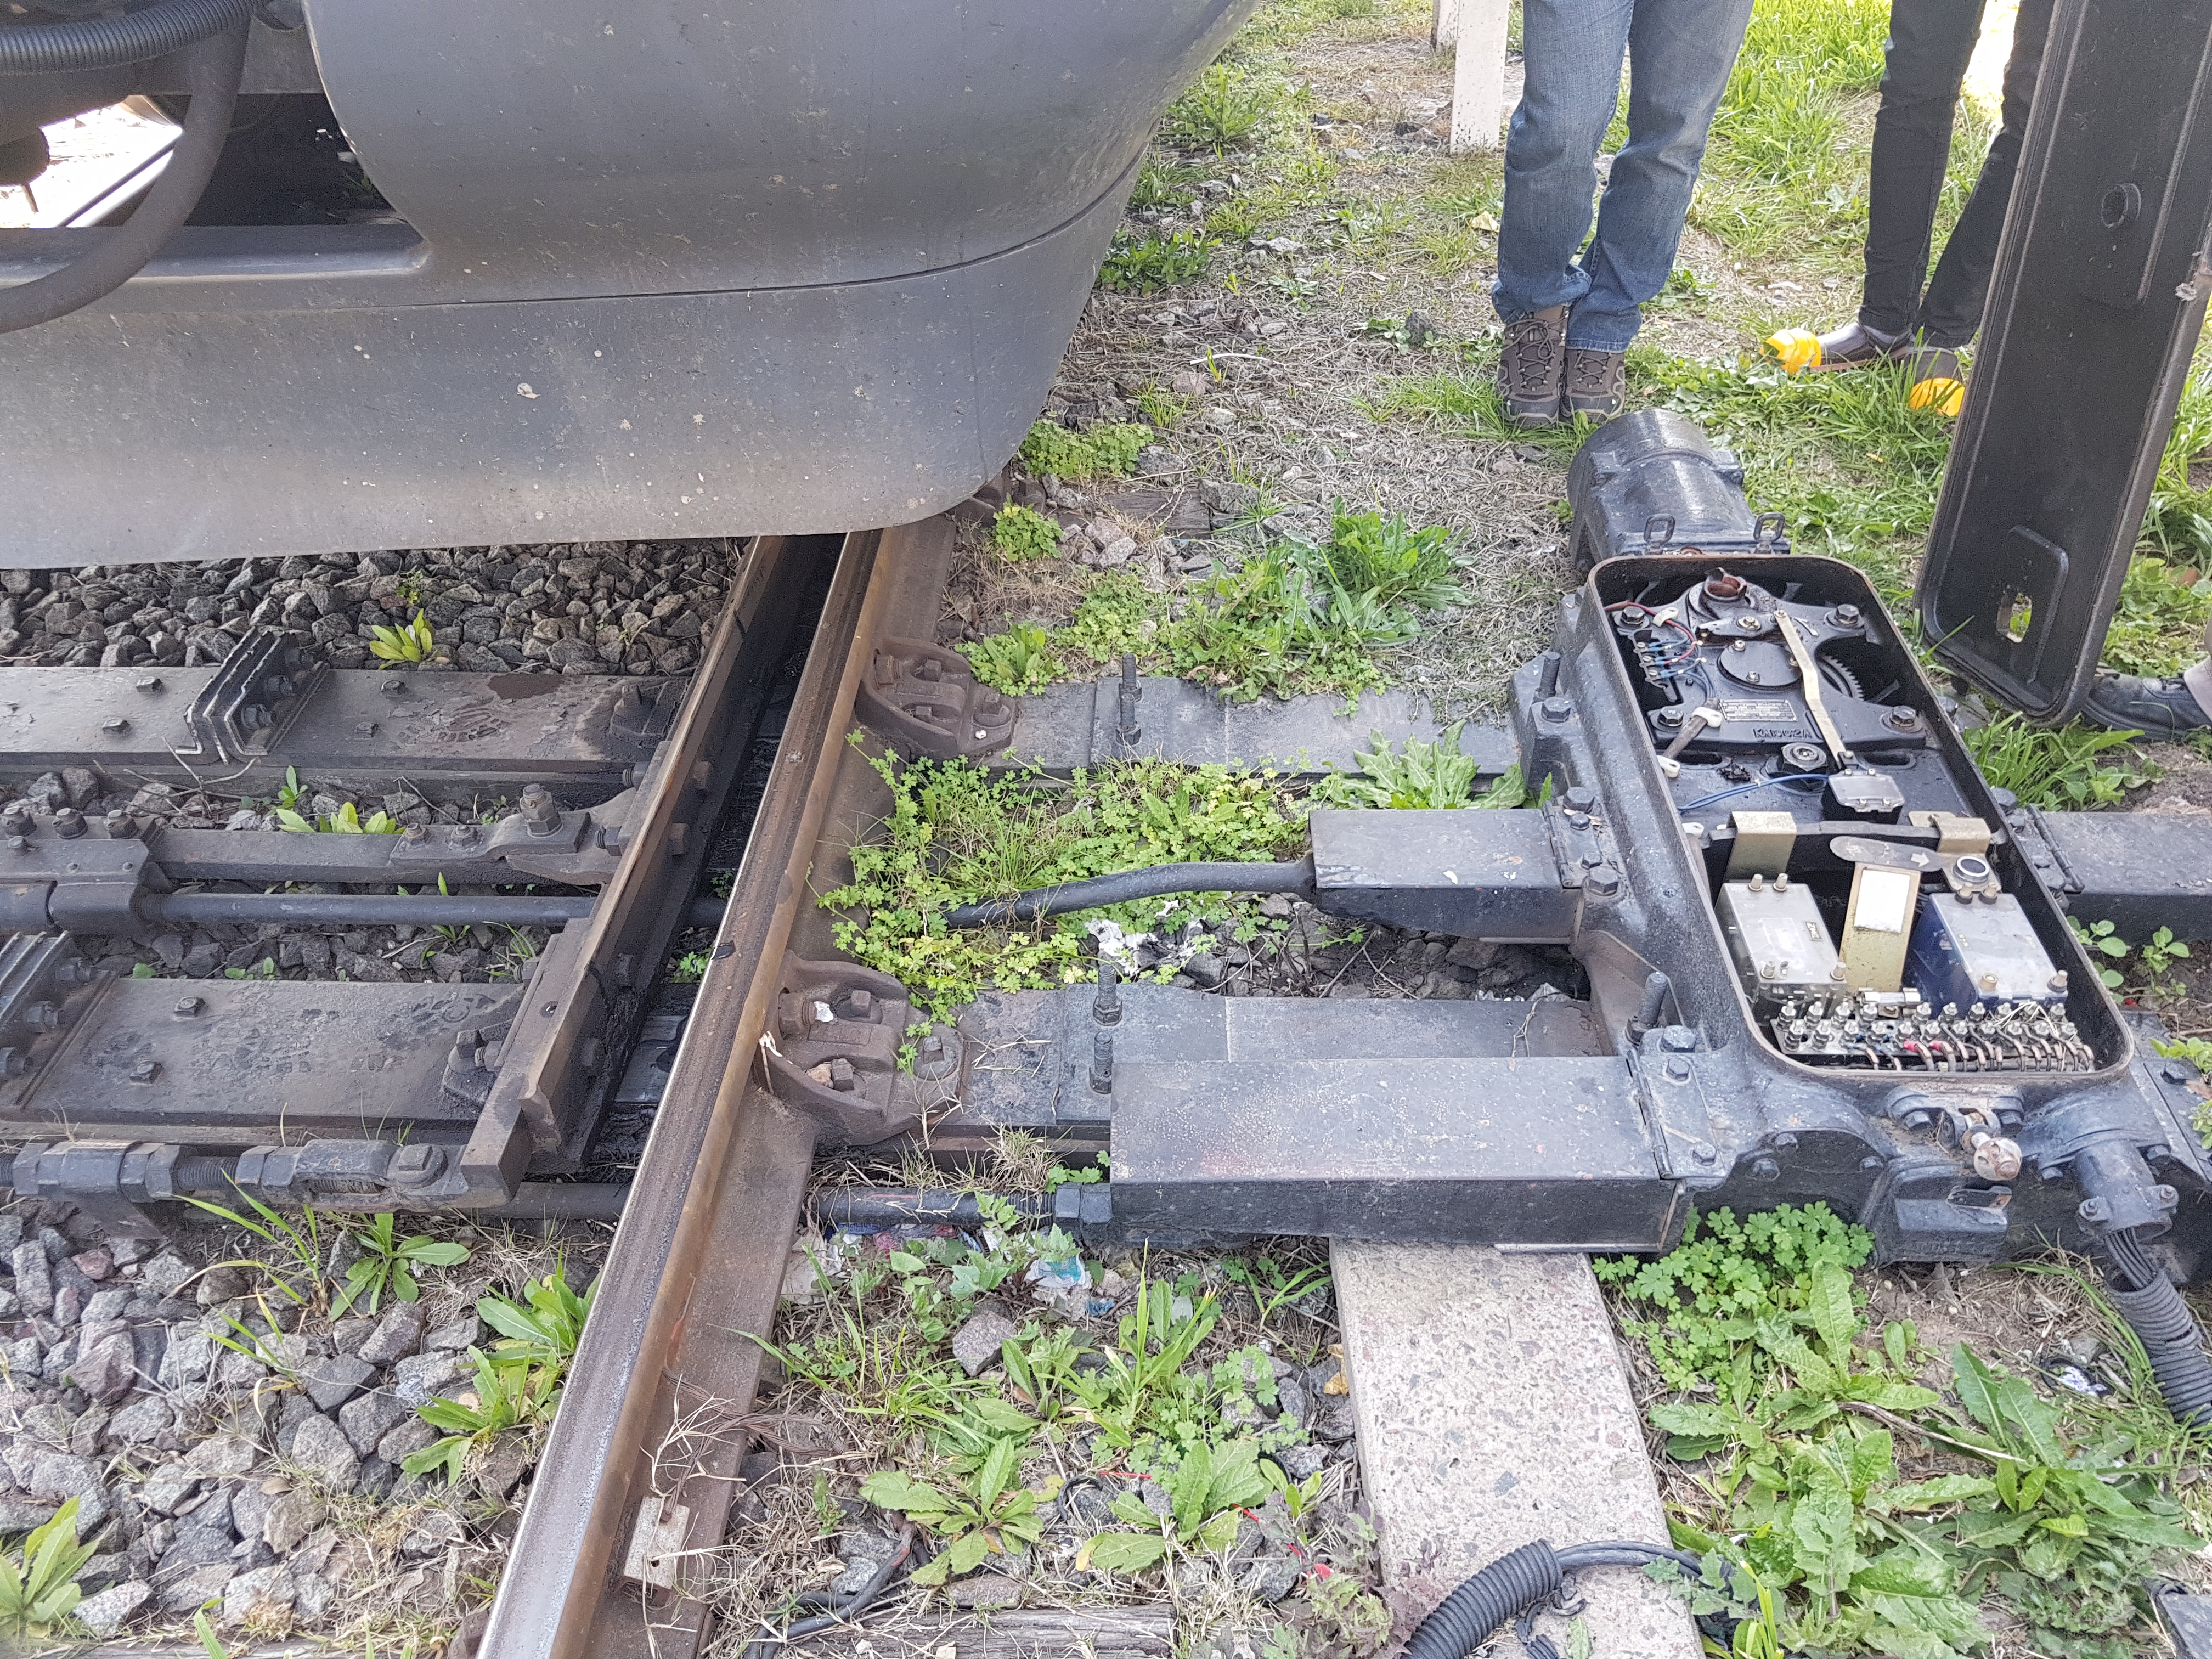
\includegraphics[width=0.75\textwidth]{Figuras/Cambios.jpg}
        \centering\caption{Máquina de cambios.}
        \label{fig:cambios_1}
    \end{figure}

    En la Figura \ref{fig:cambios_2} se muestra el cambio de vía de la estación Matheu de la Línea Mitre. Se observa que según sea la posición de la máquina de cambios, el tren puede continuar en la misma vía o hacer el cambio a la otra vía.

    \begin{figure}[H]
        \centering
        \includegraphics[width=0.75\textwidth]{Figuras/Cambios_2.jpg}
        \centering\caption{Cambio de vías de estación Matheu, Linea Mitre.}
        \label{fig:cambios_2}
    \end{figure}

    %En la Figura \ref{fig:cambios_3} se muestran las posiciones que puede adoptar el cambio. En la posición normal, los trenes pueden circular de forma directa, en paralelo, por la vía principal en sentidos opuestos. En la posición reversa, por el contrario, se permite el intercambio de trenes de una rama principal a otra en sentido opuesto o a una ramificación secundaria de la red.

   % \begin{figure}[H]
   %     \centering
   %     \includegraphics[width=1\textwidth]{Figuras/cambio_3.PNG}
   %     \centering\caption{Posiciones adoptadas por un cambio de vías simple.}
   %     \label{fig:cambios_3}
   % \end{figure}

    Al ser mecanismos que necesitan tiempo para cambiar de un estado al otro, no puede asumirse que el comando es obedecido al instante. Incluso podría darse el caso que jamás llegue a cumplirse la orden debido a desperfectos mecánicos o eléctricos. Es por eso que introducimos los conceptos de comando, indicación y correspondencia, tal como se ilustran en la Figura \ref{fig:cambios_4}.

    \begin{figure}[H]
        \centering
        \includegraphics[width=1\textwidth]{Figuras/cambios}
   \textit{}     \centering\caption{Comando, indicación y correspondencia en un cambio de vías.}
        \label{fig:cambios_4}
    \end{figure}
    
    El comando es la instrucción que el sistema de enclavamientos envía a la máquina de cambios. Esta instrucción puede ser modificar la posición de normal a reverso o de reverso a normal. La indicación es el estado que la máquina de cambios informa al sistema de enclavamientos. El sistema solo asume que el comando fue obedecido cuando tanto el comando como la indicación muestran una correspondencia. En caso contrario, el sistema de enclavamiento no puede asumir cual es el estado real del sistema, si el comando enviado o el estado reportado por la máquina de cambios. El mismo concepto puede ser aplicado en cualquier otro elemento mecánico, como por ejemplo las barreras ferroviarias.

    El RNA debe analizar diversos atributos distribuidos entre la clase \textit{switchIS} (Código \ref{lst:switchIS}), la clase \textit{spotElementProjection} (Código \ref{lst:switch}) y la clase \textit{switchIL} (Código \ref{lst:switchIL}). La clase \textit{switchIS} se encuentra dentro del vector de clases \textit{switchesIS}, dentro de la clase \textit{functionalInfrastructure}, que a su vez es parte de la clase infrastructure. La clase \textit{switchIS} define el id de la máquina de cambios, el tipo (ordinario), el \textit{netElement} al cual pertenece la entrada del cambio y hacia que lado se encuentra la vía de continuación y ramificación si transitamos desde el \textit{netElement} del cambio hacia el cambio mismo. En este caso, si transitamos por el \textit{netElement} ne16 el tren tendrá la vía de continuación en la mano derecha y la ramificación en la mano izquierda. Los cambios de vías simples ("ordinarySwitch") siempre tienen una rama izquierda y una rama derecha definida. Además, dentro de la definición de cada rama tenemos el atributo \textit{netRelationRef}, del cual se puede obtener, procesamiento mediante, los otros \textit{netElement} correspondientes a las ramas: ne15 y ne14.

    \begin{lstlisting}[language = XML, caption = Clase \textit{switchIS} , label = {lst:switchIS}]
    <switchIS id="swi84" continueCourse="right" branchCourse="left" type="ordinarySwitch">
        <name name="Sw01" language="en"/>
        <spotLocation id="swi84_sloc01" netElementRef="ne16" applicationDirection="reverse" intrinsicCoord="0.0000"/>
        <designator register="_Example" entry="SWITCH Sw01"/>
        <leftBranch netRelationRef="nr_ne15ne16_swi84" branchingSpeed="0" joiningSpeed="0" radius="-500"/>
        <rightBranch netRelationRef="nr_ne14ne16_swi84" branchingSpeed="0" joiningSpeed="0" radius="0"/>
    </switchIS>
    \end{lstlisting}

    La clase \textit{spotElementProjection} define la ubicación en el espacio del elemento ferroviario referido. En este caso, como se puede ver en el Código \ref{lst:switch}, la posición de la máquina de cambios es la coordenada (-561 ; -450).

    \begin{lstlisting}[language = XML, caption = Clase \textit{spotElementProjection} , label = {lst:switch}]
    <spotElementProjection refersToElement="swi84" id="vis01_sep16">
        <name name="Sw01" language="en"/>
        <coordinate x="-560.994" y="-450.000"/>
    </spotElementProjection>
    \end{lstlisting}

    La clase \textit{switchIL}, definida dentro del vector de clases \textit{switchesIL}, se encuentra dentro de la clase \textit{assetsForIL}, en la clase \textit{interlocking}. Contiene datos extra sobre el comportamiento dinámico del cambio de vías y define explícitamente los otros dos nodos, en contraposición a \textit{switchIS} del cual hay que obtenerlos procesando un string. El RNA puede obtener los \textit{netElement} de ambas clase y compararlos, anulando el análisis si los \textit{netElement} definidos en \textit{switchIS} y \textit{switchIL} no son coincidentes.
    
    \begin{lstlisting}[language = XML, caption = Clase \textit{SwitchIL} , label = {lst:switchIL}]
    <switchIL id="il_swi84" maxThrowTime="PT10S" typicalThrowTime="PT6S" isKeyLocked="false" returnsToPreferredPosition="false">
        <refersTo ref="swi84"/>
        <branchLeft ref="ne15"/>
        <branchRight ref="ne14"/>
    </switchIL>
    \end{lstlisting}
    
    El RNA utiliza el Algoritmo \ref{alg:switches} para detectar todos estos parámetros y crear un vector de máquinas de cambios (switches) indexado por el id de cada máquina de cambios (sw\_id). La existencia y ubicación de las máquinas de cambios ya se habían obtenido mediante el análisis de la red de grafos ferroviaria. El Algoritmo \ref{alg:switches} analiza la clase \textit{switchIS} y confirma la existencia de la máquina de cambios, para luego la clase \textit{spotElementProjection} y confirmar la ubicación de la misma. Los datos obtenidos en switches[sw\_id].LeftBranch y switches[sw\_id].RightBranch, permiten obtener los nodos de las ramificaciones que luego se conformarán analizando la clase \textit{switchIL} en algoritmos posteriores.

    \begin{algorithm}[H]\captionsetup{labelfont={sc,bf}, labelsep=newline}
            \caption{Algoritmo detector de cambios de vías.}
            \label{alg:switches}
            \begin{algorithmic}
                \STATE \{switches\} $\gets$ \{\}
                \IF {infrastructure.SwitchesIS != None} 
                    \FOR{i in infrastructure.SwitchesIS[0].SwitchIS}
                        \IF{i.Id not in switchesIS.keys()}
                            \STATE sw\_id $\gets$ i.Name[0].Name
                            \STATE j $\gets$ i.SpotLocation[0]
                            \STATE node $\gets$ j.NetElementRef
                            \STATE type $\gets$ i.Type
                            
                           	\IF{type == 'OrdinarySwitch'}
	                           	\STATE left\_id $\gets$ i.LeftBranch[0].NetRelationRef
	                           	\STATE right\_id $\gets$ i.RightBranch[0].NetRelationRef
	                           	\STATE switches[sw\_id] $\gets$ \{"Node":node\}
	                           	\STATE switches[sw\_id] $\gets$ \{"Continue":i.ContinueCourse\}
	                           	\STATE switches[sw\_id] $\gets$ \{"Branch":i.BranchCourse\}
	                           	\STATE switches[sw\_id] $\gets$ \{"Dir":j.ApplicationDirection\}
	                           	\STATE switches[sw\_id] $\gets$ \{"LeftBranch":j.left\_id\}
	                           	\STATE switches[sw\_id] $\gets$ \{"RightBranch":j.right\_id\}
                            \ENDIF
                            \IF{type == 'DoubleSwitchCrossing'}
	                            \STATE straightBranch\_A\_id $\gets$ i.StraightBranch[0].NetRelationRef
	                            \STATE straightBranch\_B\_id $\gets$ i.StraightBranch[1].NetRelationRef
	                            \STATE turningBranch\_A\_id $\gets$ i.TurningBranch[0].NetRelationRef
	                            \STATE turningBranch\_B\_id $\gets$ i.TurningBranch[1].NetRelationRef
	                            
	                            \FOR{X,Z combination(A,B)}
		                            \STATE switches[sw\_id+'XZ'] $\gets$ \{"Node":node\}
		                            \STATE switches[sw\_id+'XZ'] $\gets$ \{"Continue":i.ContinueCourse\}
		                            \STATE switches[sw\_id+'XZ'] $\gets$ \{"Branch":i.BranchCourse\}
		                            \STATE switches[sw\_id+'XZ'] $\gets$ \{"Dir":j.ApplicationDirection\}
		                            \STATE switches[sw\_id+'XZ'] $\gets$ \{"LeftBranch":j.straightBranch\_X\}
		                            \STATE switches[sw\_id+'XZ'] $\gets$ \{"RightBranch":j.turningBranch\_Z\}
	      						\ENDFOR
                            \ENDIF
                            
                        \ENDIF
                    \ENDFOR
                \ENDIF
                \STATE visual\_data $\gets$ visualization.Visualization
                \IF {visual\_data != None}
                    \FOR {i in  visual\_data[0].SpotElementProjection}
                        \STATE sw\_id $\gets$ i.Name[0].Name
                        \IF {'Sw' in sw\_id}
                            \STATE pos\_x $\gets$ int(i.Coordinate[0].X)
                            \STATE pos\_y $\gets$ int(i.Coordinate[0].Y)
                            \STATE switches[sw\_id] $\gets$ \{"Position":[pos\_x,-pos\_y]\}
                        \ENDIF 
                    \ENDFOR
                \ENDIF
            \OUTPUT \{switches\}
            \end{algorithmic}
        \end{algorithm}
    
    % SEMAFOROS
    \subsection{Semaforos}

\lipsum[1]
    \section{Redes de grafos}
    \label{sec:grafos}

    \lipsum[1]
    \section{Algoritmos de generacion de señalamiento}

\lipsum[1]

\subsection{Fin de via}

\lipsum[1]

\begin{algorithm}[hbt!]
            \caption{Line border and buffer stops algorithm}\label{alg:LBBS}
            \DontPrintSemicolon
            %\SetAlgoLined
            \SetNoFillComment
            \LinesNotNumbered 
            \For { netElement WITH BufferStops }
            {
                \If { NOT EXIST next netElement }
                {
                    [Signals] $\gets$ ADD stop signal $>>$\;
                    [Signals] $\gets$ ADD departure signal $<<$\;
                }
                \If { NOT EXIST prev netElement }
                {
                    [Signals] $\gets$ ADD stop signal $<<$\;
                    [Signals] $\gets$ ADD departure signal $>>$\;
                }
            }
            \For { netElement WITH LineBorder }
            {
                \If { netElement.Length $>$ FIXED\_LENGTH }
                {
                    \If { NOT EXIST next netElement }
                    {
                        [Signals] $\gets$ ADD departure signal $>>$\;
                    }
                    \If { NOT EXIST prev netElement }
                    {
                        [Signals] $\gets$ ADD departure signal $<<$\;
                    }
                }
            }
            \KwResult{[Signals]} 
        \end{algorithm}
\subsection{Detectores}

\lipsum[1-2]

\begin{algorithm}[hbt!]
            \caption{Train detection elements algorithm}\label{alg:RJ}
            \DontPrintSemicolon
            %\SetAlgoLined
            \SetNoFillComment
            \LinesNotNumbered 
            \For { netElement WITH AxleCounters or RailJoints }
            {
                Track.Length = Length ( between RailJoints )\;
                \If { Track.Length $>$ FIXED\_LENGTH }
                {
                    [Signals] $\gets$ ADD circulation signal $>>>$\;
                    [Signals] $\gets$ ADD circulation signal $<<<$\;
                }
            }
            \KwResult{[Signals]} 
        \end{algorithm} 

\lipsum[1]
\includegraphics{example-image}\\
\lipsum[1]
\subsection{Plataformas ferroviarias}

    % Autoridad > derecho limitado a una porcion
    % Claridad > autoridad no ambigua
    % Anticipacion > avisar con antelacion
    % Granularidad > rutas cortas y funcionales
    % Terminalidad > avisar fin de via
    % Infraestructura > avisar de infraestructura
    % No bloqueo > circulacion fluida

    En la Sección \ref{sec:platform} definimos la clase platform que modela a las plataformas ferroviarias. Las plataformas ferroviarias son un punto del recorrido donde las formaciones pueden detenerse, algunas veces de forma opcional dependiendo el itinerario, para que los pasajeros desciendan y nuevos pasajeros puedan ascender. Claramente existe una limitación de autoridad, las formaciones necesitan un nuevo permiso para continuar circulando una vez alcanzada la plataforma. Permiso que será otorgado o negado según el estado del sistema a continuación del recorrido. Las plataformas ferroviarias suelen encontrarse en zonas pobladas, cerca de otras infraestructuras, zonas comerciales o residenciales, por lo que avisar con antelación al maquinista que debe disminuir la marcha y/o detenerse es esencial.

    Además, es posible que las formaciones convivan con otras formaciones que también hacen uso de la estación, por lo que las señales deben ser unívocas y claras. Algunas estaciones pueden contener fines de vías o ramificaciones hacia talleres u otros ramales, por lo que también se aplica el principio de terminalidad y granuralidad. Finalmente, es importante el mantener una circulación fluida de las formaciones, de modo de no retrasar el itinerario de las formaciones que vienen detrás, por lo que se deberá aplicar el principio de no bloqueo.

    En el Algoritmo \ref{alg:PTF} definimos a la señal de partida como la única señal necesaria para operar una plataforma, asumiendo que la señal de ingreso de la misma será dada por otra instancia previa. De no existir otro elemento cercano por el cual se genere una señal, se puede asumir que la distancia a la plataforma es muy larga y, por lo tanto, se aplicaría el Algoritmo \ref{alg:RJ}, protegiendo a la plataforma. En el caso de que la vía se bidireccional se añadiran señales de partida para ambos sentidos.

    \begin{algorithm}[hbt!]
        \caption{Algoritmo de generación de señalamiento para platforms.}\label{alg:PTF}
        \DontPrintSemicolon
        %\SetAlgoLined
        \SetNoFillComment
        \LinesNotNumbered 
        \For { netElement WITH Platform }
        {
            \tcc{Before leaving platform from left}
            [Signals] $\gets$ ADD departure signal $\gg\gg$\;
            \tcc{After leaving platform from right}
            [Signals] $\gets$ ADD departure signal $\ll\ll$\;
        }
        \KwResult{[Signals]} 
    \end{algorithm}

    Aplicando el Algoritmo \ref{alg:PTF} a un sistema de dos vías paralelas con plataformas pertenecientes a la misma estación obtenemos el resultado ilustrado en la Figura \ref{fig:signal_platform}.Se asumieron que ambas vías son bidireccionales, en caso contrario solo se generarían las señales S01 y S02.
    
    \begin{figure}[h!]
        \centering
        \includegraphics[width=1\textwidth]{Figuras/platforms.PNG}
        \centering\caption{Señalamiento generado para estaciones ferroviarias.}
        \label{fig:signal_platform}
    \end{figure}
    
    Una formación que circule de izquierda a derecha deberá detenerse antes de la señal S01, en caso de utilizar la vía superior, o antes de la señal S04, en caso de utilizar la vía inferior. Análogamente, las formaciones deberán detenerse antes de las señales S03 y S02 en el caso de transitar de derecha a izquierda por la vía superior o inferior respectivamente. Sólo cuando estas señales otorguen a la formación autoridad para circular podrán reanudar su marcha hasta la próxima señal disponible, fuera del alcance de lo ilustrado en la Figura \ref{fig:signal_platform}.
\subsection{Cruces de via}

\lipsum[1]

\begin{algorithm}[hbt!]
            \caption{Level crossing algorithm}\label{alg:LC}
            \DontPrintSemicolon
            %\SetAlgoLined
            \SetNoFillComment
            \LinesNotNumbered 
            \For { netElement WITH LevelCrossing }
            {
                \tcc{Before reaching level crossing}
                [Signals] $\gets$ ADD circulation signal $>>>$\;
                \tcc{After leaving level crossing}
                [Signals] $\gets$ ADD circulation signal $<<<$\;
            }
            \KwResult{[Signals]} 
        \end{algorithm}
\subsection{Maquinas de cambios}

    \lipsum[1-2]

    \begin{algorithm}[hbt!]
        \caption{Switch algorithm}\label{alg:SW}
        \DontPrintSemicolon
        %\SetAlgoLined
        \SetNoFillComment
        \LinesNotNumbered 
        \For { Switch in Switches }
        {
            \tcc{All signals must point to switch}
            \Switch{ Switch.Type }
            {
                \Case{Start}
                {
                    [Signals] $\gets$ ADD circulation signal\;
                    [Signals] $\gets$ ADD maneuver signal\;
                }
                \Case{Continue branch}
                {
                    [Signals] $\gets$ ADD circulation signal\;
                }
                \Case{Detour branch}
                {
                    [Signals] $\gets$ ADD maneuver signal\;
                }
            }   
        }
        \KwResult{[Signals]} 
    \end{algorithm}

    \lipsum[1]
    \includegraphics{example-image}\\
    \lipsum[1-2]
    \section{Algoritmos de simplificacion de señalamiento}

\lipsum[1]

\subsection{Algoritmo de herencia horizontal}

    \lipsum[1-3]

    \begin{algorithm}[hbt!]
        \caption{Horizontal inheritance algorithm}\label{alg:horizontal}
        \DontPrintSemicolon
        %\SetAlgoLined
        \SetNoFillComment
        \LinesNotNumbered 
        \For{ each netElement }
        {
            \For{ each object in netElement }
            {
                \If{dist(Obj\_A,Obj\_B) $<$ MIN\_DISTANCE }
                {
                    move\_signals\_between(Obj\_A,Obj\_B)
                }
            }
        }
        \KwResult{[Signals]} 
    \end{algorithm}

    \lipsum[1-3]
\subsection{Algoritmo de simplificación por herencia vertical}
	\label{sec:vertical}
	% Autoridad > derecho limitado a una porcion
	% Claridad > autoridad no ambigua
	% Anticipacion > avisar con antelacion
	% Granularidad > rutas cortas y funcionales
	% Terminalidad > avisar fin de via
	% Infraestructura > avisar de infraestructura
	% No bloqueo > circulacion fluida
	
	Como se explicó en la Sección \ref{sec:switches}, una máquina de cambios bifurca la vía principal en dos: una vía que continúa la rama principal y otra vía que se convierte en una rama secundaria. Tanto la vía de continuación como la vía ramificada pueden tener otra máquina de cambios que, a su vez, vuelve a dividir el trazado ferroviario en dos. Esto incrementa más y más el nivel de complejidad de la red, añadiendo caminos divergentes al principal que luego, mas adelante, podrían, o no, volver a converger utilizando mas máquinas de cambios. Cada divergencia aporta un nivel de profundidad a la red, mientras que cada convergencia reduce en uno el nivel de profundidad.
	
	Una máquina de cambios que tiene en cualquiera de sus ramas divergentes el nodo de inicio de otra máquina de cambios a una distancia pequeña es un cambio compuesto. Los cambios compuestos requieren considerar a ambas máquinas de cambios como una sola, ya que es necesario posicionar ambos mecanismos para completar un movimiento. El ejemplo de La Figura \ref{fig:signal_vertical_1} ayudará a clarificar el concepto de cambios compuestos e introducir el Algoritmo de simplificación por herencia vertical.	

	\begin{figure}[h!]
		\centering
		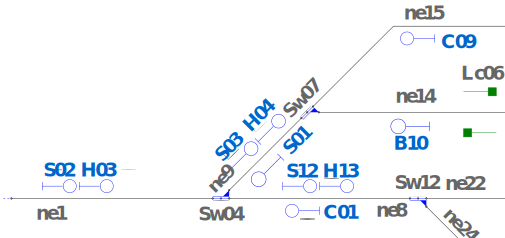
\includegraphics[width=1\textwidth]{Figuras/Figure8_Crop.pdf}
		\centering\caption{Señalamiento generado, simplificado por algoritmo de herencia vertical.}
		\label{fig:signal_vertical_1}
	\end{figure}
	
	En la Sección \ref{sec:signal_switches} se introdujo el Algoritmo \ref{alg:SW} que define la asignación de señalamiento para los cambios de vías: una señal de circulación (S) y de maniobra (H) para el nodo de inicio (S), una señal de circulación para el nodo de continuación (C) y una señal de maniobras para el nodo de desvío (B). El Algoritmo \ref{alg:SW} se aplicó de forma independiente a las máquinas de cambios Sw04, Sw07 y Sw12 y se obtuvo el señalamiento de la Figura \ref{fig:signal_vertical_1}. No obstante, el señalamiento generado no cumple con el principio de no bloqueo, al situar las señales S03, H04, B01, S12, H13 y C01 en las secciones correspondientes a los netElements ne9 y ne8. De esa manera, las formaciones podrían detenerse en esas secciones si las mencionadas señales presentasen un aspecto rojo.
	
	Una formación detenida en la sección correspondiente al netElement ne9 no permitiría mover el cambio de vía Sw04, al tener parte de la formación aún en ne1. Tampoco permitiría accionar el cambio de vías Sw07 al no haber finalizado el movimiento. Análogamente para una formación detenida en la sección correspondiente al netElement ne8. Es necesario que el movimiento finalice, despejando las secciones y permitiendo que otras formaciones utilicen los cambios de vías Sw04 y Sw07, o cualquier combinación de mas de un cambio de vías.
	
	Para solucionar el problema expuesto, el RNA aplica el Algoritmo \ref{alg:vertical} de simplificación por herencia vertical para reposicionar las señales situadas en zonas conflictivas. A diferencia del señalamiento explicado en la Sección \ref{sec:generacion}, las señales que protegen a un cambio de vías B situado en una rama mas profunda de la red no se encuentran inmediatamente precediendo al cambio de vías B. Estas señales son movidas a ramas de menor profundidad con suficiente espacio físico para contenerlas, situándose precediendo a otro cambio de vías A que decimos que ha \emph{heredado} el señalamiento del cambio de vía B.
		
	\begin{algorithm}[hbt!]
        \caption{Algoritmo de simplificación por herencia vertical}\label{alg:vertical}
        \DontPrintSemicolon
        %\SetAlgoLined
        \SetNoFillComment
        \LinesNotNumbered 
        \For{ each Signal protecting a Sw\_A }
        {
            \For{each Sw\_B != Sw\_A}
            {
                \tcc{Criteria \#0}
                \If{distance(Sw\_A,Sw\_B) $>$ MIN\_DISTANCE}
                {
                    Continue\;
                }
                \If{S in Sw\_A.Branch also in Sw\_B.Start} 
                {
                   \tcc{Criteria \#1}
                   \If{S points to Sw\_B.Start}
                   {
                        Move S to Sw\_A.Start\;
                   }
                   \tcc{Criteria \#2}
                   \If{S points to Sw\_A.Branch}
                   {
                        Move S to Sw\_B.Continue\;
                        Move S to Sw\_B.Branch\;
                   }
                }
                \If{S in Sw\_A.Continue also in Sw\_B.Start}
                {
                   \tcc{Criteria \#3}
                   \If{S points to Sw\_B.Start}
                   {
                        Move S to Sw\_A.Start\;
                   }
                   \tcc{Criteria \#4}
                   \If{S points to Sw\_A.Continue}
                   {
                        Move S to Sw\_B.Continue\;
                        Move S to Sw\_B.Branch\;
                   }
                }
            }
        
        }
        \KwResult{[Signals]} 
    \end{algorithm}

    Como puede apreciarse en el Algoritmo \ref{alg:vertical}, existen cinco criterios a considerar para aplicar la herencia vertical. El primer criterio es excluyente, si la distancia entre ambas máquinas de cambios supera un parámetro determinado entonces el algoritmo no se aplica, al existir suficiente distancia para situar el señalamiento sin generar obstrucciones debido a formaciones detenidas entre ambos. Cuando la distancia entre las máquinas de cambios es menor a lo esperado, se aplican los otros cuatro criterios, en función de que nodos conectan entre sí la vía que comparten.
    
    Definiendo al cambio de vías A como el cambio principal y el cambio de vías B como el cambio secundario situado en alguna de las ramificaciones del cambio de vías A, podemos diferenciar dos casos: que el señalamiento se encuentre en la rama de continuación del cambio de vías A o se encuentre en la rama de desvío. A su vez, este señalamiento puede estar apuntando al cambio de vías A o al cambio de vías B, protegiéndolo respectivamente. 
    
    El criterio para el desplazamiento del señalamiento busca cumplir el principio de Anticipación, el principio de Infraestructura y el principio de no bloqueo. Para eso, las señales son adelantadas, desplazándolas en sentido opuesto al que apuntan. Si el señalamiento se encuentra en la rama de desvío o continuación del cambio de vías A es indistinto, lo importante es a donde apuntan las señales. Si estas apuntan hacia el nodo de inicio del cambio de vías B, deben ser desplazadas, sin alterar su cantidad, hacia el nodo de inicio del cambio de vías A. 
    
    En el caso particular de que las señales en la zona conflictiva apunten hacia el cambio de vías A, tanto a su nodo de desvío como al nodo de continuidad, las mismas deberían moverse en sentido contrario al que apuntan. Pero en esa dirección la red se ramifica en dos debido al cambio de vías B. En este caso, las señales mueven duplicadas, a la rama de continuación y a la rama de desvío del cambio de vías B, en su totalidad.
    
    Aplicando el Algoritmo \ref{alg:vertical} de herencia vertical al ejemplo de la Figura \ref{fig:signal_vertical_1} obtenemos el señalamiento de la Figura \ref{fig:signal_vertical_2}. Las señales S03, H04, B01, S12, S13 y C01 serán adelantadas para despejar las secciones correspondientes a los netElements ne9 y ne8. Debido a esto, los tres cambios de vías se usarán de forma complementaria, creando los siguientes cambios compuestos: $Sw_{04}^R+Sw_{07}^N$, $Sw_{04}^R+Sw_{07}^R$, $Sw_{04}^N+Sw_{12}^N$ y $Sw_{04}^N+Sw_{12}^R$. Los cuales se leen, considerando el ejemplo del cambio compuesto $Sw_{04}^R+Sw_{07}^N$, de la siguiente manera: el cambio de vías Sw04 en posición normal y el cambio de vías Sw07 en posición reversa.
    
    \begin{figure}[h!]
    	\centering
    	\includegraphics[width=1\textwidth]{Figuras/Figure9_Crop.pdf}
    	\centering\caption{Señalamiento generado, simplificado por algoritmo de herencia vertical.}
    	\label{fig:signal_vertical_2}
    \end{figure}
    
    En el caso de las señales S03 y H04 que apuntan al nodo de inicio del cambio de vías Sw07, son desplazadas en sentido contrario al que apuntan, aplicando el criterio \#1. Estas señales son movidas hasta el nodo de continuación del cambio de vías Sw04, correspondiente al netElement ne1, protegiendo el inicio del cambio compuesto $Sw_{04}^R+Sw_{07}^N$ y $Sw_{04}^R+Sw_{07}^R$ . A estas señales se le suman las señales S12 y H13 situadas en la sección correspondiente al netElement ne8 que, aplicando el criterio \#3, son desplazadas al nodo de inicio del cambio de vías Sw04, protegiendo el inicio del cambio compuesto $Sw_{04}^N+Sw_{12}^N$ y $Sw_{04}^N+Sw_{12}^R$.
    
    La señal B01 apunta al nodo de desvío del cambio de vías Sw04 y, por el criterio \#2, debe ser duplicada y movida. Una señal se posiciona en la sección correspondiente al netElement ne15 y la otra a la sección asociada al netElement ne14. De esta manera, la señal S01a y S01b seguirán protegiendo el nodo de desvío del cambio de vías Sw04, pero previamente tendrán que hacer uso del cambio de vías Sw07 en cualquiera de sus dos posiciones, protegiendo los nodos de cambio y continuación del cambio compuesto $Sw_{04}^R+Sw_{07}^N$ y $Sw_{04}^R+Sw_{07}^R$. De igual manera, la señal C01 es movida y duplicada a las secciones correspondientes a los netElements ne22 y ne24, debido al criterio \#4. Estas nuevas señales C01a y C01b continúan protegiendo el nodo de continuación del cambio de vías Sw04, pero ahora deberán, adicionalmente, hacer uso del cambio de vías Sw12, protegiendo los nodos de continuación y desvío del cambio compuesto $Sw_{04}^N+Sw_{12}^N$ y $Sw_{04}^N+Sw_{12}^R$.
    
    El Algoritmo \ref{alg:vertical} de herencia vertical es exitoso a la hora de despejar las zonas críticas entre cambios de vías muy cercanos. No obstante, también incrementa la cantidad de señales, como en el caso de las señales S01 y C01 al ser desplazadas en sentido divergente por los cambios de vías Sw07 y Sw12. Además, el Algoritmo \ref{alg:vertical} de herencia vertical no es aplicable solo a una dupla de cambios de vías, sino que puede ser aplicado para cualquier conjunto de cambios de vías. Esto provoca que las señales se hereden de forma iterativa hasta encontrar un cambio de vías con suficiente espacio para albergar las señales. Debido a esto, la cantidad de señales al comienzo de un cambio de vías previo a una ramificación profunda de la red tendrá una gran cantidad de señales.
    
    En el caso del ejemplo de las Figuras \ref{fig:signal_vertical_1} y \ref{fig:signal_vertical_2}, el algoritmo concluye con seis señales en el nodo de inicio de los cuatro cambios compuestos. Estas seis señales deberán habilitar cuatro caminos a transitar desde ne1: hacia ne15, hacia ne14, hacia ne22 y hacia ne24. Es claro que, teniendo mas señales que caminos a habilitar, será necesario un algoritmo de limpieza de señales duplicadas y/o que ya no tengan una utilidad en el señalamiento. El proceso de simplificación es explicado en profundidad en la Sección \ref{sec:limpieza}.
\subsection{Limpieza de señales}

Prioridad y repetición
\lipsum[1]

\begin{algorithm}[hbt!]
        \caption{Signal reduction algorithm}\label{alg:reduction}
        \DontPrintSemicolon
        %\SetAlgoLined
        \SetNoFillComment
        \LinesNotNumbered 
        Sources = $\{$ T,L,S,B,P,C,J,X $\}$\;
        \For{ Sig\_A \& Sig\_B in [Signals]}
        {
            \If{ A != B  \& Sig\_A.From == Sig\_B.From }
            {
             CDL\_zones.Pos = detect\_next\_dangers ( Sig\_A )\;
             A.Pos,B.Pos = Sig\_A.Pos,Sig\_B\;
             Safe = zone\_between(CDL\_zones.Pos,A.Pos,B.Pos)\;
                 \If{ NOT safe }
                 {
                    \If{ $|A.Pos,B.Pos|$ $<$ MIN\_DISTANCE }
                    {
                        \If{ Sig\_A \& Sig\_B same orientation }
                        {
                            \If{ Sig\_A \& Sig\_B same direction }
                            {
                                \If { Sig\_A \& Sig\_B type "Circ" }
                                {
                                    \If{ Sig\_A.Idx $<$ Sig\_B.Idx }
                                    {
                                        delete Sig\_B  else Sig\_A
                                    }
                                    %{
                                    %    delete( Sig\_A )
                                    %}
                                }
                            }
                        }
                        \If{ Sig\_A \& Sig\_B different source}
                        {
                            delete\_lowest\_priority( Sig\_A,Sig\_B )\;
                        }
                    }
                }
            }
        }
        \KwResult{[Signals]} 
    \end{algorithm}

    \lipsum[1-3]

    \section{Generación de tablas de enclavamiento}

	\label{sec:rutas}
	
	% Once the signalling is generated and simplified, it is necessary to establish the railway routes to create the railway interlocking table. A railway route is the simplest path between two consecutive signals in the same direction, using the same tracks \cite{SIGNALLING_1,AUTOMATIC_SIMPLE_SIGNAL}. The route may contain switches, level crossings, platforms or any railway element within the path. A railway route is defined with a start and an end signal, accompanied by the indication of the corresponding safe state of the railway netElements like switches or level crossings and the tracks assigned (P1, P2, P3, P4, P5, P6, P7). Algorithm \ref{alg:routes} describes the mechanisms to detect and assign routes.
	
	\lipsum[1-5]
	
	\begin{algorithm}[hbt!]
        \caption{Route detection algorithm}\label{alg:routes}
        \DontPrintSemicolon
        %\SetAlgoLined
        \SetNoFillComment
        \LinesNotNumbered 
        Routes = []\; 
        route = 0\;
        \For{ start in [Signals] }
        {
            \tcc{Find manoeuvre and circulation signals}
            \If{ start != "Stop" }
            {
                dir = start\_sig.Direction\;
                \tcc{Find next signal w/ same direction}
                
                end = find\_next\_signal(start,[Signals])\;

                [paths] = find(start.node,end.node,graph)\;
                
                \For{ node in [paths] }
                {
                    \tcc{Find rail objects within path}
                    sws = find(graph[node],switches)\;
                    lc = find(graph[node],levelCrossings)\;
                    ptf = find(graph[node],platforms)\;
                    %route ++\;
                    Routes[route++] = $\{$start,end,dir,node,sws,lc,ptf$\}$\;
                }
            }
        }
        \KwResult{[Routes]} 
    \end{algorithm}
    
    %Stop signals cannot be starting signals and, therefore, are ignored, considering only circulation and manoeuvre signals. It is necessary to follow the graph network in the same direction as the starting signal to identify all the incoming signals through all the possible paths from the netElement where the starting signal is. For example, three routes were highlighted in Figure \ref{fig:Routes} over the simplified signalling for Example 1, with signal S22 as the starting signal: S22 to S32, S22 to X15 and S22 to T05.
    
    \lipsum[1-2]
    
    \begin{figure}[h]
    	\centering
    	\includegraphics[width=1\textwidth]{Figuras/Figure11.pdf}
    	\centering\caption{Signalling simplified in Example 1 with three routes indicated.}
    	\label{fig:Routes}
    \end{figure}
    
    %Having the start signal and all the end signals, it is necessary to identify the main rail objects within those paths, such as switches (their position), level crossings (that must be closed), platforms and tracks. In Example 1 (Figure \ref{fig:Routes}), a route defined by signals S22 and T05 covers tracks ne1, ne9 and ne15 using switch Sw04 in reverse position and switch Sw07 in normal position without any level crossing is involved.
    
    %If two routes share the same start signal or end signal they are conflicting routes. The same if they share one netElement, switch, level crossing or the same signals swapped. It means both routes cannot be approved at the same time, one of them being approved implies the others must be blocked until the first one was completed or cancelled. Two routes could have the same start and end signal but use different tracks, but they cannot be approved at the same time because there must be necessary a switch within that routes, with opposite positions and only one position can be approved when one route is ongoing. Conflicting routes are indicated in the interlocking table that is automatically generated by the RNA. Every route is created based on the created graph network and the shortest path algorithm for directed graphs. The paper \cite{GRAPH_4_ROUTES} explores another approach to finding routes based on interlocking tables.
    
    \lipsum[1-3]
    \section{Validación de tablas de enclavamiento}

	\lipsum[1-5]
	
	
	\begin{algorithm}[hbt!]
		\caption{Algoritmo de validación de tablas de enclavamiento ferroviarias.}\label{alg:interlocking_tables}
		\DontPrintSemicolon
		%\SetAlgoLined
		\SetNoFillComment
		\LinesNotNumbered 
		old\_graph = create\_Digraph()\; 
		new\_graph = create\_Digraph()\; 
		\tcc{Create digraphs for both interlocking tables}
		\For{start\_net,end\_net,old\_route in old\_table}
		{
			old\_graph $\Leftarrow$ start\_net,end\_net,old\_route\;
		}
		\For{start\_net,end\_net,new\_route in new\_table}
		{
			new\_graph $\Leftarrow$ start\_net,end\_net,new\_route\;
		}
		
		\tcc{Detect coincidences between both digraphs}
		routes\_found = 0\;
		\For{start\_net,end\_net,old\_route in old\_table}
		{
			\If{start\_net != end\_net}
			{
				routes\_found += find\_shortest\_paths(start\_net , end\_net)\;
			}
			\Else
			{
				\If{start\_net in new\_graph}
				{
					routes\_found += 1\;
				}
				\Else
				{
					\If{end\_net in new\_graph}
					{
						begin\_nodes = List(neighbours of end\_net in new\_graph)\;
						
						\If{begin\_nodes != []}
						{
							routes\_found += find\_shortest\_paths(begin\_nodes[0] , end\_net)\;
						}
					}
				}
			}
		
		}

		\KwResult{routes\_found} 
	\end{algorithm}
	
	\lipsum[1-5]
    \section{Comprobación de principios de señalamiento ferroviario}
	\label{sec:validar_principios}
	
	% Autoridad > todas las rutas combinadas cubren toda la traza ferroviaria.
	% Claridad > autoridad no ambigua.
	% Anticipacion > avisar con antelacion.
	% Granularidad > rutas cortas y funcionales.
	% Terminalidad > avisar fin de via.
	% Infraestructura > avisar de infraestructura.
	% No bloqueo > circulacion fluida.
				
	En esta sección se abordará el proceso de validación de cada uno de los principios ferroviarios establecidos en la Sección \ref{sec:principios}, como parte del proceso expuesto en la Sección \ref{sec:validacion}. Para ello, serán abordados de manera genérica cada uno de los principios de señalamiento junto con el algoritmo que el RNA utiliza para validarlo, previo a exportar el señalamiento generado.
	
	\subsection{Comprobación del principio de autoridad}
		% Autoridad > todas las rutas combinadas cubren toda la traza ferroviaria.
		
		El principio de autoridad radica en que las rutas otorgan a las formaciones un permiso de uso limitado para circular por las vías. No obstante, la combinación de todas las autoridades disponibles de ser otorgadas deben cubrir la totalidad de la traza ferroviaria. Es decir, no debe existir ninguna sección de vía que se encuentre fuera del alcance de las rutas y, por lo tanto, aislada de la red. Puede darse el caso de que una sección de vía tenga una ruta de entrada o de salida, pero no ambas. También puede darse el caso de que la sección de vía sea transitada, pero no sea ni inicio ni final de ninguna ruta.
		
		El RNA utiliza el Algoritmo \ref{alg:ppio_autoridad} para validar el principio de autoridad comparando los netElements alcanzados por las rutas disponibles, con la lista de netElements potenciales de ser alcanzados. Esta última salvedad deja fuera las secciones de vías que preceden a una señal de circulación posterior a un final de vía relativo (lineBuffer). Esto se realiza ya que estas secciones de vía son transitadas por rutas fuera de la locación bajo análisis, rutas que terminan en la señal de circulación mencionada.

		\begin{algorithm}[H]
			\caption{Algoritmo de validación del principio de autoridad.}\label{alg:ppio_autoridad}
			\DontPrintSemicolon
			%\SetAlgoLined
			\SetNoFillComment
			\LinesNotNumbered 
			Validated = False\;
			$\{$Routes$\}$, $\{$netElements$\}$ without netElements with lineBuffer\; 
			\tcc{Validate that every route covers all the railway tracks.}
			\For{route in $\{$Routes$\}$}
			{
				\If{route[begin] in $\{$netElements$\}$}
				{
					Remove route[begin] from $\{$netElements$\}$\; 
				}
				\If{route[end] in $\{$netElements$\}$}
				{
					Remove route[end] from $\{$netElements$\}$\; 
				}
				\For{track in route[paths]}
				{
					\If{track in $\{$netElements$\}$}
					{
						Remove track from $\{$netElements$\}$\; 
					} 
				}
			}
			\If{$\{$netElements$\}$ is Empty}
			{
				Validated = True\; 
			} 
			\KwResult{Validated} 
		\end{algorithm}
		
		Se asume inicialmente que la validación es fallida por defecto. Si al finalizar el Algoritmo \ref{alg:ppio_autoridad} no existe ningún netElement remanente en la lista, se considera que la validación es exitosa.	
			
	\subsection{Comprobación del principio de claridad}
		% Claridad > autoridad no ambigua
		
		El principio de claridad radica en que el señalamiento no posee señales ambiguas. Es decir, no existen dos rutas distintas que otorguen autoridad sobre las mismas secciones de vía, en el mismo sentido, utilizando la misma infraestructura. En otras palabras, las rutas en una misma dirección y sentido no se solapan, cada una comienza donde otra ha terminado.
		
		El RNA utiliza el Algoritmo \ref{alg:ppio_claridad} para validar el principio de claridad, generando una red de grafos dirigidos. La misma se constituye utilizando todas las rutas definidas por el RNA como aristas, y a los netElements que conectan como nodos de la red. Si se detecta que existen dos rutas R$^{\prime}$ y R$^{\prime\prime}$ que conectan dos nodos A y B en el mismo sentido, utilizando la misma infraestructura, entonces se dice que las rutas son ambiguas y el principio de claridad no se cumple.
		
		\begin{algorithm}[H]
			\caption{Algoritmo de validación del principio de claridad.}\label{alg:ppio_claridad}
			\DontPrintSemicolon
			%\SetAlgoLined
			\SetNoFillComment
			\LinesNotNumbered 
			Validated = False\;
			$\{$Routes$\}$\; 
			\tcc{Validate that every netElement is reached by one route only.}
			\For{route in $\{$Routes$\}$}
			{
				begin = route[begin]\;
				end = route[end]\;
				index = route[index] \;
				direction = route[direction]\;
				digraph = create\_digraph(begin,end,index,direction)\;	
			}
			\If{digraph has no redundant routes}
			{
				Validated = True\;
			}
			\KwResult{Validated} 
		\end{algorithm}
		
		Aunque el orden de validación de los principios de señalamiento es indistinto, la confirmación de que las señales son suficientes para alcanzar toda la red (Principio de autoridad) y de que no existen señales ambiguas (Principio de claridad) facilita las siguientes validaciones. Esto se debe a que, con estas dos comprobaciones, ya sabemos que contamos con la mínima cantidad de señales para recorrer la red de forma unívoca, garantizando la correcta logística de la red. Los siguientes principios son necesarios para validar la seguridad del señalamiento generado por el RNA.
		
	\subsection{Comprobación del principio de anticipación}
		% Anticipacion > avisar con antelacion
		
		El principio de anticipación radica en que existe una señal previo a cada peligro, situada en la zona de señalamiento. Una zona señalamiento puede estar próxima a una curva, al final de la traza ferroviaria o en las inmediaciones de un paso a nivel, una estación, un cambio de vías o cualquier infraestructura ferroviaria a ser protegida. En otras palabras, el señalamiento debe estar distribuido de tal manera que entre dos señales que constituyen una ruta exista un único peligro o situación que quiera la atención del conductor.
		
		El RNA utiliza el Algoritmo \ref{alg:ppio_anticipacion} para validar el principio de anticipación, detectando las regiones de señalamiento como zonas peligro peligrosas, producto del trazado ferroviario (curvas, finales de vía) o de la infraestructura ferroviaria (plataformas, pasos a nivel, etc.). 
		
		\begin{algorithm}[H]
			\caption{Algoritmo de validación del principio de anticipación.}\label{alg:ppio_anticipacion}
			\DontPrintSemicolon
			%\SetAlgoLined
			\SetNoFillComment
			\LinesNotNumbered 
			Validated = True, $\{$Dangers$\}$ = None\;
			$\{$Routes$\}$, $\{$Track$\}$\; 
		
			\tcc{Validate that each danger is protected by the signalling.}
			
			\For{curve in $\{$Tracks$\}$}
			{
				$\{$Dangers$\}$ $\Leftarrow$ ADD curve
			}
			
			\For{element in $\{$Infraestructure$\}$}
			{
				$\{$Dangers$\}$ $\Leftarrow$ ADD element
			}
			
			\For{danger in $\{$Dangers$\}$}
			{
				
				\For{track going into danger}
				{
					\If{track has signal AND signal points to danger}
					{
						Continue\;
					}
					\Else
					{
						Validated = False\; 
						Stop iterations\;
					}
				}	
			}
			
			\KwResult{Validated} 
		\end{algorithm}
		
		A continuación, el Algoritmo \ref{alg:ppio_anticipacion} comprueba que existe una señal para cada dirección del peligro, apuntando en el sentido del mismo. Garantizando de esta forma, que previo a cada peligro inicie o finalice una ruta, en caso de que la ruta sea segura de ser transitada o no, respectivamente.
		
		Una sola región de señalamiento que tenga una de sus entradas sin proteger por una señal es suficiente para que el Algoritmo \ref{alg:ppio_anticipacion} devuelva un resultado negativo. Si todas las entradas de cada región de señalamiento están protegidas por una señal, entonces el principio de anticipación se encuentra cumplido. En el caso de que los elementos ferroviarios se encuentren muy próximos, por herencia horizontal, se consideran un único elemento y sus regiones de señalamiento se simplifican como se explicó en la Sección \ref{sec:horizontal}.
		
	\subsection{Comprobación del principio de granularidad}
		% Granularidad > rutas cortas y funcionales
		
		El principio de granularidad radica en que las rutas deben ser lo suficientemente cortas como para permitir una logística flexible, pero no tan cortas como para no tener ninguna funcionalidad real. Consideramos, por lo tanto, que el señalamiento debe estar distribuido de tal forma que las rutas tengan una funcionalidad básica. Entre éstas funciones tenemos el uso de un elemento ferroviario específico (o conjunto de elementos ferroviarios, si están muy próximos) o la subdivisión de rutas cuyos tramos originales eran demasiado extensos.
		
		El RNA utiliza el Algoritmo \ref{alg:ppio_granularidad} para validar el principio de granularidad, analizando que elementos ferroviarios se encuentran contenidos en cada ruta y la distancia entre las señales que conforman la misma. Se recorre el listado de rutas generadas por el RNA, que ya establece los elementos contenidos en las rutas, las señales que las definen y la posición de las mismas. En cada ruta se analiza si existen elementos ferroviarios que justifiquen la existencia de la ruta y si el largo de la misma se encuentra entre un rango mínimo y máximo estipulado. Si alguna de estas condiciones se cumple, entonces se procede a analizar la siguiente ruta. En caso contrario, el Algoritmo \ref{alg:ppio_granularidad} finaliza de forma negativa. Si todas las rutas analizadas superan el proceso, entonces el principio de granularidad ha sido validado exitosamente.
		
		\begin{algorithm}[H]
			\caption{Algoritmo de validación del principio de granularidad.}\label{alg:ppio_granularidad}
			\DontPrintSemicolon
			%\SetAlgoLined
			\SetNoFillComment
			\LinesNotNumbered 
			Validated = True\;
			$\{$Routes$\}$\; 
			\tcc{Validate that each route has a purpose and a min/max length.}
			\For{route in $\{$Routes$\}$}
			{
				\If{MIN $>$ route[length] $>$ MAX OR route[elements] == None}
				{
					Validated = False\; 
					Stop iterations\;
				}				
			}
			\KwResult{Validated} 
		\end{algorithm}
		
		Si la ruta es demasiado pequeña o demasiado larga, la validación finaliza de forma negativa. Si la ruta tiene un tamaño adecuado pero no contiene ningún elemento relevante de ser protegido, también se rechaza la validación. En caso contrario, si todas las rutas cumplen el criterio entonces se da por validado el principio de granularidad.
		
	\subsection{Comprobación del principio de terminalidad}
		% Terminalidad > avisar fin de via
		
		El principio de terminalidad radica en que el señalamiento debe indicar, sin excepciones, el final de cada rama del trazado ferroviario, sin importar si es un final relativo u absoluto. Como se explicó en la Sección \ref{sec:bufferstop}, tanto los finales de vía relativos como los absolutos necesitan una señal de parada que permita habilitar la salida de la formación de la locación bajo estudio. Además, los finales de vía absolutos requieren de una señal de partida para reiniciar la marcha de la formación en la dirección contraria, retomando el recorrido dentro de la traza ferroviaria.	
		
		El RNA utiliza el Algoritmo \ref{alg:ppio_terminalidad} para validar el principio de terminalidad, recorriendo cada una de las rutas generadas y analizando aquellas que culminan o empiezan en un final de vía. Una vez detectadas las rutas que posean lineBorders o bufferStops, se procede a analizar que clase de señales poseen. Si son compatibles con las condiciones indicadas en la Sección \ref{sec:bufferstop}, entonces se continúa analizando con la siguiente ruta. Caso contrario, la validación termina de forma negativa. Si todas las rutas analizadas superan el proceso, entonces el principio de terminalidad ha sido validado exitosamente.
		
		\begin{algorithm}[H]
			\caption{Algoritmo de validación del principio de terminalidad.}\label{alg:ppio_terminalidad}
			\DontPrintSemicolon
			%\SetAlgoLined
			\SetNoFillComment
			\LinesNotNumbered 
			Validated = True\;
			$\{$Routes$\}$\; 
			\tcc{Validate that each lineBorder and BufferStop have protective signals}
			\For{route in $\{$Routes$\}$}
			{
				\If{lineBorder in route[element] and route goes to lineBorder}
				{
					\If{signal is not route[end]}
					{
						Validated = False\;
					}
				}
				
				\If{bufferStop in route[element]}
				{
					\If{route goes to bufferStop and signal is not route[end]}
					{
						Validated = False\;
					}
					\If{route start from bufferStop and signal is not route[begin]}
					{
						Validated = False\;
					}
				}
			}
			
			\KwResult{Validated} 
		\end{algorithm}
		
		Este principio es el más sencillo de validar positivamente ya que, por como fue diseñado el RNA, tanto los \textit{lineBorder} y los \textit{bufferStop} siempre tendrán señalamiento y dichas señales tienen la máxima prioridad, por lo que no pueden simplificarse con otras señales. No obstante, si el usuario elige de forma explícita no generar señales para estos elementos ferroviarios, entonces este principio de señalamiento podría no cumplirse.		
				
	\subsection{Comprobación del principio de infraestructura}
		% Infraestructura > avisar de infraestructura
		
		El principio de infraestructura radica en que el señalamiento debe proteger, sin excepciones, toda infraestructura ferroviaria crítica, tales como las plataformas y los pasos a nivel. Con excepción de los cambios de vías, que son cubiertos por el principio de no bloqueo. La infraestructura deberá estar protegida por el señalamiento tal como se explicó en la Sección \ref{sec:platform} y la Sección \ref{sec:crossing}, permitiendo a las formaciones detenerse en las plataformas y antes de los pasos a nivel, respectivamente.

		El RNA utiliza el Algoritmo \ref{alg:ppio_infraestructura} para validar el principio de infraestructura, recorriendo cada una de las rutas generadas y analizando aquellas que atraviesan paso a nivel o que inician o finalizan en una plataforma. 
		
		\begin{algorithm}[H]
			\caption{Algoritmo de validación del principio de infraestructura.}\label{alg:ppio_infraestructura}
			\DontPrintSemicolon
			%\SetAlgoLined
			\SetNoFillComment
			\LinesNotNumbered 
			Validated = True\;
			$\{$Routes$\}$\; 
			\tcc{Validate that each platform and crossing have protective signals}
			\For{route in $\{$Routes$\}$}
			{
				\If{platform in route[element]}
				{
					\If{route goes across platform and signal is not route[end]}
					{
						Validated = False\;
					}
					\If{route start from platform and signal is not route[begin]}
					{
						Validated = False\;
					}
				}
				
				\If{levelCrossing in route[element]}
				{
					\If{route goes to levelCrossing and signal is not route[end]}
					{
						Validated = False\;
					}
					\If{route start before levelCrossing and signal is not route[begin]}
					{
						Validated = False\;
					}
				}
			}
			
			\KwResult{Validated} 
		\end{algorithm}
		
		Una vez detectadas las rutas, se procede a analizar que clase de señales poseen.  Si son compatibles con las condiciones indicadas en la Sección \ref{sec:platform} y la Sección \ref{sec:crossing}, entonces se continúa analizando con la siguiente ruta. Caso contrario, la validación termina de forma negativa. Si todas las rutas analizadas superan el proceso, entonces el principio de infraestructura ha sido validado exitosamente.
		
		En el caso de que las plataformas y los pasos a nivel se encuentren muy próximos, por la simplificación de señalamiento por herencia horizontal explicada en la Sección \ref{sec:horizontal}, igualmente el Algoritmo \ref{alg:ppio_infraestructura} buscará las señales mas próximas al nuevo elemento ferroviario compuesto. De esta manera, al analizar todas las rutas exitosamente, es posible validar el señalamiento que protege a los elementos ferroviarios críticos, cumpliendo el principio de infraestructura.
		
	\subsection{Comprobación del principio de no bloqueo}
		% No bloqueo > circulacion fluida
		
		El principio de no bloqueo radica en que el señalamiento debe proteger los cambios de vías en sus tres direcciones: inicio, normal y desvío, como se explica en la Sección \ref{sec:switches}. A su vez, debe garantizarse que los cambios compuestos no tengan señales intermedias, para evitar que las formaciones se detengan en zonas críticas, bloqueando los cambios de vías para otras formaciones que las requieran, como se explica en la Sección \ref{sec:vertical}.
		
		El RNA utiliza el Algoritmo \ref{alg:ppio_nobloqueo} para validar el principio de no bloqueo, recorriendo la lista de máquinas de cambios. El primer paso es agrupar en tres listas distintas todos los netElements de cada cambio de vía según su dirección: inicio, normal y desvío. Luego, son removidas de las listas de inicio y normal todos los netElements que también pertenezcan a la lista de desvío. De esta manera, el algoritmo contempla a los cambios compuestos productos de la simplificación por herencia vertical (ver Sección \ref{sec:vertical}). 
		
		\begin{algorithm}[H]
			\caption{Algoritmo de validación del principio de no bloqueo.}\label{alg:ppio_nobloqueo}
			\DontPrintSemicolon
			%\SetAlgoLined
			\SetNoFillComment
			\LinesNotNumbered 
			Validated = False\;
			$\{$Switches$\}$\;
			switch\_start = [], switch\_normal = [], switch\_branch = [], critical = []\;
			\tcc{Validate that each switch have protective signals}
			
			\tcc{List netElements for each side of each switch}
			
			\For{sw in $\{$Switches$\}$}
			{
				switch\_start $\leftarrow$ ADD sw[netElement] for 'Start'\;
				switch\_normal $\leftarrow$ ADD sw[netElement] for 'Normal'\;
				switch\_branch $\leftarrow$ ADD sw[netElement] for 'Branch'\;
			}	
			
			\tcc{Remove netElements that also belongs to a branch}
			\For{sw in $\{$Switches$\}$}
			{
				switch\_start $\leftarrow$ REMOVE netElement if in switch\_branch\;
				switch\_normal $\leftarrow$ REMOVE netElement if in switch\_branch\;
				critical $\leftarrow$ ADD netElement in switch\_branch AND (switch\_start OR switch\_normal)\;
			}	
			
			\tcc{Remove the netElements that have signals}
			\For{netElement that has a signal}
			{
				\If{netElement in unprotected\_switch\_start}
				{
					switch\_start $\leftarrow$ REMOVE netElement\;
				}
				
				\If{netElement in unprotected\_switch\_normal}
				{
					switch\_normal $\leftarrow$ REMOVE netElement\;
				}
			}
			
			\tcc{Final condition}
			\If{switch\_start == [ ] AND switch\_normal == [ ] AND critical has no signals}
			{
				Validated = True\;
			}
			
			\KwResult{Validated} 
		\end{algorithm}
		
		A continuación, se remueven de las listas de inicio y normal todos los netElements que tienen una señal apuntando hacia el cambio de vías. Finalmente, si ambas listas se encuentran vacías y los netElements de la lista de cambios que también perteneciesen a las listas de inicio y normal originales no tienen señales, entonces el principio de no bloqueo ha sido validado exitosamente.
		
	Una vez que todos los principios de señalamiento ferroviario han sido validados podemos afirmar que el señalamiento generado por el RNA es seguro y cumple con todos los requisitos planteados en la Sección \ref{sec:principios}. Dicho señalamiento deberá ser implementado por el Generador Automático de Códigos en VHDL (ACG), explicado en profundidad en la Sección \ref{sec:ACG}.
